\documentclass[12pt,a4paper]{article} 

\usepackage{fn2kursstyle}
\usepackage[russian]{babel}
\usepackage[T2A]{fontenc} 
\usepackage[utf8]{inputenc} 
%\usepackage{geometry}
\usepackage{mathtools}
\usepackage{tikz}
\usepackage{chngcntr}
\usepackage{float}
\usepackage[most]{tcolorbox} % для управления цветом
\counterwithout{equation}{section}
\counterwithout{figure}{section}
\frenchspacing 

\makeatletter
\newcommand*{\rom}[1]{\expandafter\@slowromancap\romannumeral #1@}
\makeatother

\title{Метод конечных элементов в задаче моделирования прогиба балки}
\group{ФН2-61Б}
\author{К.\,А.~Касьянова}
\supervisor{И.\,К.~Марчевский}
\date{2022}

\newcommand*\circled[1]{\tikz[baseline=(char.base)]{
            \node[shape=circle,draw,inner sep=2pt] (char) {#1};}}

\makeatletter
\newenvironment{sqcases}{%
  \matrix@check\sqcases\env@sqcases
}{%
  \endarray\right.%
}
\def\env@sqcases{%
  \let\@ifnextchar\new@ifnextchar
  \left\lbrack
  \def\arraystretch{1.2}%
  \array{@{}l@{\quad}l@{}}%
}
\makeatother

\def\Arsh{\mathop{\mathrm{Arsh}}}

\graphicspath{{legacy/}, {../pic/}}

\begin{document}
    \maketitle
	\tableofcontents
	\pagebreak

	\section{Введение и постановка задачи}
	Работа посвящена методам решения дифференциального уравнения 4-го порядка, описывающего форму упругой линии балки. Получены аналитические решения, в числе прочего, использующие функцию Хевисайда, а также численные решения, полученные методом конечных элементов.

	Проанализирована точность метода конечных элементов, проанализированы порядки точности, которые наблюдаются при использовании двух и трехузловых конечных элементов в зависимости от того, какой степенью гладкости обладает функция внешней нагрузки: гладкая, непрерывная, но негладкая, разрывная, но ограниченная и  сосредоточенной.  В рамках метода конечных элементов получены выражения для функций форм и компонент матриц жёсткости для двухузлового и трехузлового балочного элемента.

	Дифференциальное уравнение, описывающее форму упругой линии балки в наиболее общей постановке является нелинейным, в нём фигурирует кривизна, вычисляемая по формуле: 
	$$ \varkappa = \frac{y''}{\sqrt{1+y'^{2}}^{3}}.$$
	Если прогиб балки сравнительно мал, т.е. $(y')^{2} \ll 1$, то можно принять, что $\varkappa \approx y''$ и тогда линеаризованное уравнение, описывающее прогиб балки, имеет вид:
	\begin{equation}
	(EIy^{''}_{zz})^{''}_{zz}=q,
	\label{v1}
	\end{equation}
	где $E$ --- модуль упругости балки; $I$ --- момент инерции относительно поперечной оси; $q$ --- распределённая внешняя нагрузка, действующая на балку. \\
 
Данное уравнение должно быть дополнено четырьмя граничными условиями, в качестве которых могут выступать следующие: 
\begin{enumerate}
\item[1)] $y|_{z=z_{0}}=y_{0}$ --- заданная величина прогиба;
\item[2)] $y'|_{z=z_{0}}=y'_{0}$ --- заданный угол поворота сечения;
\item[3)] $EIy''|_{z=z_{0}}=M_{0}$ --- изгибающий момент;
\item[4)] $EIy'''|_{z=z_{0}}= Q_{0}$ --- перерезывающая сила.
\end{enumerate}


\section{Метод конечных элементов}
Метод конечных элементов является одним из наиболее распространённых методов численного решения краевых задач, как для уравнений матеематической физики, так и обыкновенных. Его популярность объясняется тем, что данный метод является универсальным и технологичным: он применим для решения широкого класса задач, при этом алгоритм остаётся неизменным, что позволяет положить его в основу крупных программных комплексов инженерного анализа. 

В методе конечных элементов численное решение разыскивается в конечномерном пространстве и представляется непрерывной функцией, которая является линейной комбинацией финитных базисных функций, называемых функциями формы. 

\subsection{Двухузловой конечный элемент}
Решим дифференциальное уравнение четвёртого порядка, описывающее прогиб балки, методом конечных элементов:\\
$$(EIy^{''}_{xx})^{''}_{xx}=q,$$%
где $E$ -- модуль упругости балки, $I$ -- момент инерции поперечного сечения относительно оси $x$, $q$ -- внешняя нагрузка, действующая на балку. \\%

Рассмотрим слабую постановку задачи о прогибе (метод Галёркина):\\
\begin{equation}
	\normalsize\int\limits_{0}^{L}w\frac{d^{2}}{dz^{2}}\left(EI\frac{d^{2}u}{dz^{2}}\right)dz=\int\limits_{0}^{L}wqdz,
	\label{beam1}
\end{equation}  
где $w$ --- произвольная пробная функция, принадлежащая классу $W_{2}^{2}[0,\,L]$.
	
Полученное выражение два раза интегрируем по частям: \\
$$w\frac{d}{dz}\left(EI\frac{d^{2}u}{dz^{2}}\right)\bigg|_0^L-\int\limits_{0}^{L}\frac{dw}{dz}\frac{d}{dz}\left(EI\frac{d^{2}u}{dz^{2}}\right)dz=\int\limits_{0}^{L}wqdz,$$
$$w\frac{d}{dz}\left(EI\frac{d^{2}u}{dz^{2}}\right)\bigg|_0^L-\frac{dw}{dz}\left(EI\frac{d^{2}u}{dz^{2}}\right)\bigg|_0^L+\int\limits_{0}^{L}EI\frac{d^{2}w}{dz^{2}}\frac{d^{2}u}{dz^{2}}dz=\int\limits_{0}^{L}wqdz.$$

Область интегрирования разделим на $N_e$ участков длины  $L_e$, каждый из которых нызывается конечным элементом.

\begin{figure}[H]
		\centering
		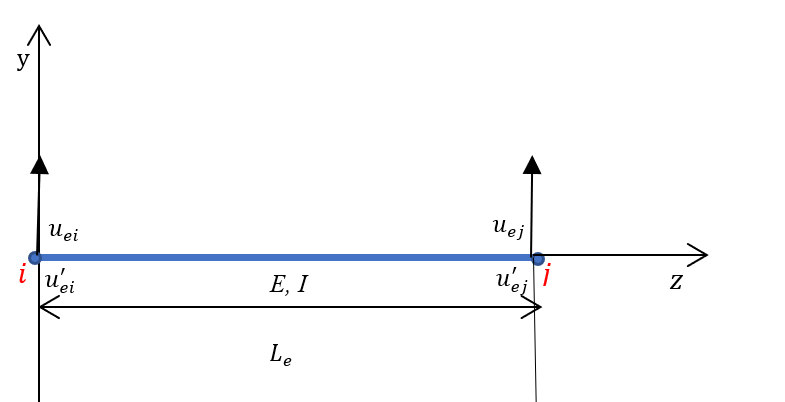
\includegraphics[width=0.65\textwidth]{element}
		\caption{}
		\label{fig:element}
\end{figure}

Решение на каждом конечном элементе зададим линейной комбинацией базисных функций $N_{1e}(z)\ldots N_{4e}(z)$, при этом сами базисные функции выберем такими, чтобы коэффициентами при них были перемещения двух узлов конечного элемента и производные (углы поворота). Такие базисные функции называются функциями формы. 
Решение на элементе и его производная имеют вид:
	\begin{equation}
	u_e(z)=N_{1e}u|_i + N_{2e}\frac{du}{dz}\Bigr|_i+N_{3e}u|_{i+1} + N_{4e}\frac{du}{dz}\Bigr|_{i+1},
	\label{beam2}
	\end{equation} 
	\begin{equation}
\frac{du_e}{dz}=\frac{dN_{1e}}{dz}u|_i+\frac{dN_{2e}}{dz}\frac{du}{dz}\Bigr|_i+\frac{dN_{3e}}{dz}u|_{i+1}+\frac{dN_{4e}}{dz}\frac{du}{dz}\Bigr|_{i+1}.
	\label{beam3}
	\end{equation} 
	
Из условий\rem{Поправить} $u_e(0)=u|_i$, $u_e^{'}(0)=u^{'}|_{i+1}$, $u_{e}(L_e)=u|_{i+1}, u_{e}^{'}(L_e)=u^{'}|_{i+1}$ находим 
$$N_{1e}(0)=1,~ N_{1e}^{'}(0)=0,~ N_{1e}(L_e)=0,N_{1e}^{'}(L_e)=0,$$ 
$$N_{2e}(0)=0,~ N_{2e}^{'}(0)=1,~ N_{2e}(L_e)=0,N_{2e}^{'}(L_e)=0,$$ 
$$N_{3e}(0)=0,~ N_{3e}^{'}(0)=0,~ N_{3e}(L_e)=1,N_{3e}^{'}(L_e)=0,$$
$$N_{4e}(0)=0,~ N_{4e}^{'}(0)=0,~ N_{4e}(L_e)=0,N_{4e}^{'}(L_e)=1.$$

 Интегрируя данные уравнения, получаем выражения для функций формы $N_{1e},N_{2e},N_{3e},N_{4e}$:
$$N_{1e}(z)=1-\frac{3z^{2}}{L_e^{2}}+\frac{2z^{3}}{L_e^{3}}=\frac{(L_e-z)^2(L_e+2z)}{L_e^3},$$
$$N_{2e}(z)=z-\frac{2z^{2}}{L_e}+\frac{z^{3}}{L_e^{2}}=\frac{z(L_e-z)^{2}}{L_e^{2}},$$
$$N_{3e}(z)=\frac{3z^{2}}{L_e^{2}}-\frac{2z^{3}}{L_e^{3}}=\frac{z^{2}(3L_e-2z)}{L_e^3},$$
$$N_{4e}(z)=-\frac{z^{2}}{L_e}+\frac{z^{3}}{L_e^{2}}=\frac{z^2(z-L_e)}{L_e^{2}}.$$

Графики функций формы для конечного элемента длиной $L=1$ изображены на рис.~\ref{fig:hermite}.

\begin{figure}[H]
		\centering
		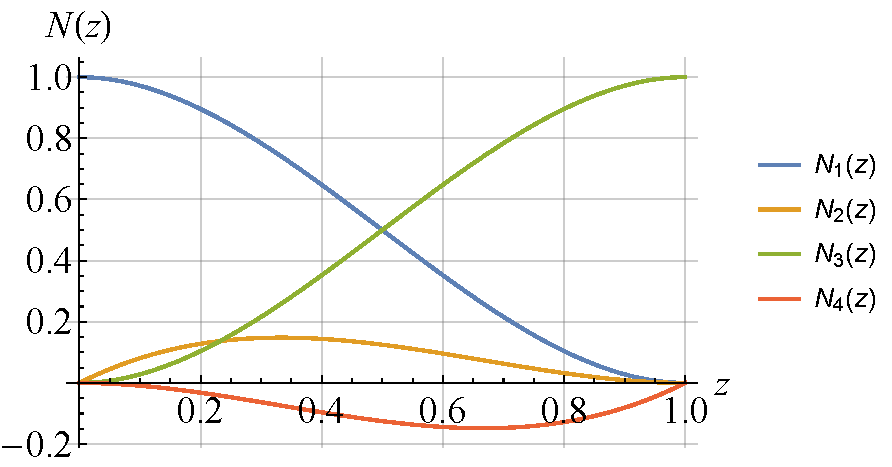
\includegraphics[scale=0.7]{hermiteVar}
		\caption{Функции формы}
		\label{fig:hermite}
	\end{figure}

Выражение (\refeq{beam2}) для функции $u_{e}$ можем записать для одного элемента в матричном виде:
$$u_e(z)=\textbf{N}_e \textbf{u}_{e}=
\left[
  \begin{array}{cccc}
     N_{1e}(z) & N_{2e}(z) & N_{3e}(z) & N_{4e}(z)
  \end{array}
\right]
\left\{
  \begin{array}{ccc}
    u_{1e}   \\
     u^{'}_{1e}  \\
		u_{2e}\\
		u^{'}_{2e}\\
  \end{array}
\right\}$$

В качестве пробных функций будем использовать функции, представимые в том же виде: 
$$w_e(z)=\textbf{N}_e \textbf{w}_{e}=
\left[
  \begin{array}{cccc}
     N_{1e}(z) & N_{2e}(z) & N_{3e}(z) & N_{4e}(z)
  \end{array}
\right]
\left\{
  \begin{array}{ccc}
    w_{1e}   \\
     w^{'}_{1e}  \\
		w_{2e}\\
		w^{'}_{2e}\\
  \end{array}
\right\}$$

Дважды продифференцировав выражения для $u_e$ и $w_e$, получим:
\[
\frac{d^{2}u_e}{dz^{2}}=\frac{d^{2}}{dz^{2}}\textbf{N}_e \textbf{u}_e=\textbf{B}_e \textbf{u}_e, \qquad
\frac{d^{2}w_e}{dz^{2}}=\frac{d^{2}}{dz^{2}}\textbf{N}_e \textbf{w}_e=\textbf{B}_e \textbf{w}_e.
\]


Тогда можно ввести следующее обозначение для вторых производных:
\begin{multline*}
\textbf{B}_e=\frac{d^{2}}{dz^{2}}\textbf{N}_e=
\left[
  \begin{array}{cccc}
     N_{1e}^{''}(z) & N_{2e}^{''}(z) & N_{3e}^{''}(z) & N_{4e}^{''}(z)
  \end{array}
\right]= {}\\
{}=\begin{bmatrix}
     \displaystyle-\frac{6}{L_e^{2}}+\frac{12z}{L_e^{3}} &  \displaystyle-\frac{4}{L_e}+\frac{6z}{L_e^{2}} &   \displaystyle\frac{6}{L_e^{2}}-\frac{12z}{L_e^{3}} &  \displaystyle-\frac{2}{L_e}+\frac{6z}{L_e^{2}}
\end{bmatrix}.
\end{multline*}

Заметим, что вторые производные от функций формы --- линейные функции. 

После подстановки полученных выражений в уравнение (\refeq{beam1}),соответствующее слабой постановке задачи, получим:
$$\sum\limits_{e=1}^{N_{e}}\int\limits_{0}^{L_e}(\textbf{B}_e\textbf{w}_e)^{T}EI(\textbf{B}_e\textbf{u}_e)dz=\textbf{w}^{T}\biggl(\sum\limits_{e=1}^{N_e}\underbrace{\int\limits_{0}^{L_e}(\textbf{B}_e)^{T}EI\textbf{B}_e dz}_{\textbf{K}_e}\biggr)\textbf{u}.$$
		
Тогда матрица жесткости для элемента $\textbf{K}_e$ имеет вид:
$$\textbf{K}_e=\int\limits_{0}^{L_e}EI\textbf{B}_e^{T}\textbf{B}_e dz.$$

Проинтегрировав данное выражение, получим:
$$\textbf{K}_e=\frac{EI}{L_e^{3}}
\left[
  \begin{array}{cccc}
    12 & 6L_e & -12 & 6L_e\\
    6L_e & 4L_e^{2} & -6L_e & 2L_e^{2}\\
		12 & -6L_e & 12 & -6L_e\\
		6L_e & 2L_e^{2} & -6L_e & 4L_e^{2}\\
  \end{array}
\right].
$$

Правая часть уравнения, соответствующая слабой постановке задачи (\refeq{beam1}) имеет следующий вид:
$$\int\limits_{0}^{L}wq(z)dz=\sum\limits_{e=1}^{N_e}\int\limits_{0}^{L_e}\textbf{w}_e^{T}\textbf{N}^T_e q(z)dz=\textbf{w}^{T}\sum\limits_{e=1}^{N_e} \int\limits_{0}^{L_e}\textbf{N}_e^{T}q(z)dz.$$

Так как слабая форма верна для любых $\textbf{w}$  окончательно запишем следующее:
 $$\textbf{Ku}=\sum\limits_{e=1}^{N_e}\int\limits_{0}^{L_e}\textbf{N}_{e}^{T}q(z)dz.$$


\subsection{Трёхузловой конечный элемент}

Область интегрирования разделим на $N_e$ участков длины  $L_e$ так, что на каждом ищется решение задачи о прогибе балки в форме (\refeq{beam1}). Данный участок называется элементом.

\begin{figure}[H]
		\centering
		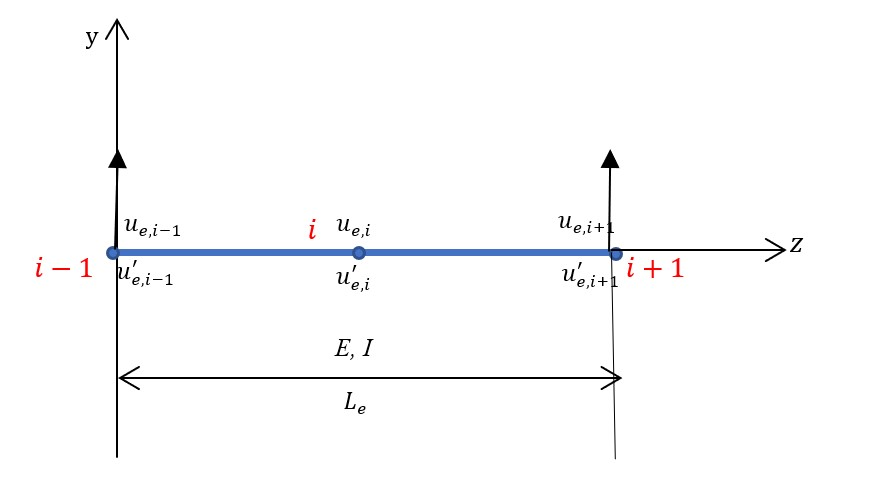
\includegraphics[width=0.8\textwidth]{threedot}
		\caption{}
		\label{fig:threedot}
	\end{figure}

Форму конечного элемента задаём линейной комбинацией базисных функций \\
$N_{1e}(z)\ldots N_{6e}(z)$, при этом сами базисные функции выберем такими, чтобы коэффициентами при них были перемещения трёх узлов конечного элемента и производные (повороты). Такие базисные функции называются функциями формы. 

\begin{equation}
	u_e(z)=N_{1e}u|_{i-1}+N_{2e}\frac{du}{dz}\Bigr|_{i-1}+N_{3e}u|_{i}+N_{4e}\frac{du}{dz}\Bigr|_{i}+N_{5e}u|_{i+1}+N_{6e}\frac{du}{dz}\Bigr|_{i+1}
	\label{beamthree1}
	\end{equation} 
	
	\begin{equation}
\frac{du_e}{dz}=\frac{dN_{1e}}{dz}u|_{i-1}+\frac{dN_{2e}}{dz}\frac{du}{dz}\Bigr|_{i-1}+\frac{dN_{3e}}{dz}u|_{i}+\frac{dN_{4e}}{dz}\frac{du}{dz}\Bigr|_{i}+\frac{dN_{5e}}{dz}u|_{i+1}+\frac{dN_{6e}}{dz}\frac{du}{dz}\Bigr|_{i+1}
	\label{beamthree2}
	\end{equation} 
	
	
Из условий $u_e(0)=u_{e, i-1},~ u_e^{'}(0)=u^{'}_{e, i-1},~ u_{e}(\frac{L_e}{2})=u_{e,i},~ u_{e}^{'}(\frac{L_e}{2})=u^{'}_{e,i},\\
 u_{e}(L_e)=u_{e,i+1},~ u_{e}^{'}(L_e)=u^{'}_{e,i+1}$ и
условий на функции формы, аналогичных таковым для двухузлового элемента,
%$$N_{1e}(0)=1,~ N_{1e}^{'}(0)=0,~ N_{1e}(\frac{L_e}{2})=0,~ N^{'}_{1e}(\frac{L_e}{2})=0,~ N_{1e}(L_e)=0,~ N_{1e}^{'}(L_e)=0,$$
%$$N_{2e}(0)=0,~ N_{2e}^{'}(0)=1,~ N_{2e}(\frac{L_e}{2})=0,~ N^{'}_{2e}(\frac{L_e}{2})=0,~ N_{2e}(L_e)=0,~ N_{2e}^{'}(L_e)=0,$$ 
%$$N_{3e}(0)=0,~ N_{3e}^{'}(0)=0,~ N_{3e}(\frac{L_e}{2})=1,~ N^{'}_{3e}(\frac{L_e}{2})=0,~ N_{3e}(L_e)=0,~ N_{3e}^{'}(L_e)=0,$$
%$$N_{4e}(0)=0,~ N_{4e}^{'}(0)=0,~ N_{4e}(\frac{L_e}{2})=0,~ N^{'}_{4e}(\frac{L_e}{2})=1,~ N_{4e}(L_e)=0,~ N_{4e}^{'}(L_e)=0,$$
%$$N_{5e}(0)=0,~ N_{5e}^{'}(0)=0,~ N_{5e}(\frac{L_e}{2})=0,~ N^{'}_{5e}(\frac{L_e}{2})=0,~ N_{5e}(L_e)=1,~ N_{5e}^{'}(L_e)=0,$$
%$$N_{6e}(0)=0,~ N_{6e}^{'}(0)=0,~ N_{6e}(\frac{L_e}{2})=0,~ N^{'}_{6e}(\frac{L_e}{2})=0,~ N_{6e}(L_e)=0,~ N_{6e}^{'}(L_e)=1.$$
получаем выражения для функций формы $N_{1e}$, $N_{2e}$, $N_{3e}$, $N_{4e}$, $N_{5e}$, $N_{6e}$:
$$N_{1e}(z)=\frac{66z^{3}}{L_e^{3}}-\frac{23z^{2}}{L_e^{2}}-\frac{68z^{4}}{L_e^{4}}+\frac{24z^{5}}{L_e^{5}}+1= \frac{4}{L^5}\Bigl( z-\frac{L_e}{2} \Bigr)^2(z-L)^2(L+6z),$$
$$N_{2e}(z)=z-\frac{6z^{2}}{L_e}+\frac{13z^{3}}{L_e^{2}}-\frac{12z^{4}}{L_e^{3}}+\frac{4z^{5}}{L_e^{4}}=\frac{}{L_e^4}=\frac{z (L-2 z)^2 (L-z)^2}{L^4},$$
$$N_{3e}(z)=\frac{16z^{2}}{L_e^{2}}-\frac{32z^{3}}{L_e^{3}}+\frac{16z^{4}}{L_e^{4}}=\frac{16 z^2 \left(z-L_e\right){}^2}{L_e^4},$$
$$N_{4e}(z)=\frac{32z^{3}}{L_e^{2}}-\frac{8z^{2}}{L_e}-\frac{40z^{4}}{L_e^{3}}+\frac{16z^{5}}{L_e^{4}}=\frac{8 z^2 \left(z-L_e\right){}^2 \left(2 z-L_e\right)}{L_e^4},$$
$$N_{5e}(z)=\frac{7z^{2}}{L_e^{2}}-\frac{34z^{3}}{L_e^{3}}+\frac{52z^{4}}{L_e^{4}}-\frac{24z^{5}}{L_e^{5}}=-\frac{z^2 \left(6 z-7 L_e\right) \left(L_e-2 z\right){}^2}{L_e^5},$$
$$N_{6e}(z)=\frac{5z^{3}}{L_e^{2}}-\frac{z^{2}}{L_e}-\frac{8z^{4}}{L_e^{3}}+\frac{4z^{5}}{L_e^{4}}=\frac{z^2 \left(z-L_e\right) \left(L_e-2 z\right){}^2}{L_e^4}.$$  

Графики функций формы для конечного элемента длинной $L=1$ изображены на рис.~\ref{fig:3_formfunctions}.

\begin{figure}[H]
		\centering
		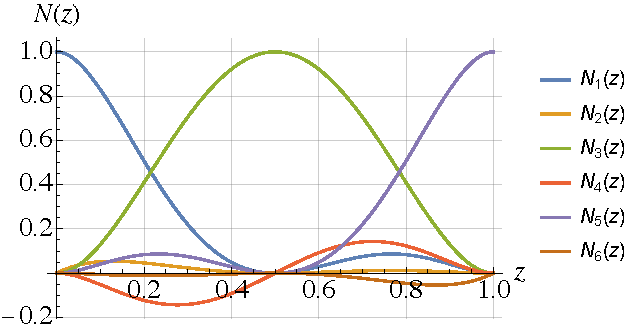
\includegraphics[width=0.6\textwidth]{3_formfunctions.pdf}
		\caption{Функции формы для трёхузлового конечного элемента длинной $L_{e}=1$}
		\label{fig:3_formfunctions}
	\end{figure}

Выражение (\refeq{beam2}) для функции $u_{e}$ можем записать в матричном виде:
\[
	u_e(x,z)=\textbf{N}_e \textbf{u}_{e}=
	\left[
	\begin{array}{ccc}
		N_{1e}(z) & \ldots & N_{6e}(z)
	\end{array}
	\right]
	\left\{
	\begin{array}{ccccccc}
		u_{1e}  &
		u^{'}_{1e}  &
		u_{2e} &
		u^{'}_{2e} &
		u_{3e} &
		u^{'}_{3e} &
	\end{array}
	\right\}^T
\]

Дальнейшие рассуждения аналогичны таковым для двухузлового элемента. Проделав соотвествующие выкладки и вычислив интегралы от вторых производных функций формы (которые теперь являются кубическими полиномами)
%
%В качестве пробных будем использовать функции, представимые в том же виде: 
%$$w_e(z)=\textbf{N}_e \textbf{w}_{e}=
%\left[
%  \begin{array}{ccc}
%     N_{1e}(z) & \ldots & N_{6e}(z)
%  \end{array}
%\right]
%\left\{
%  \begin{array}{cccccc}
%    w_{1e}   &
%     w^{'}_{1e}  &
%		w_{2e} &
%		w^{'}_{2e} &
%		w_{3e} &
%		w^{'}_{3e} &
%  \end{array}
%\right\}$$
%
%Дважды продифференцировав выражения для $u_e$ и $w_e$, получим:
%$$\frac{d^{2}u_e}{dz^{2}}=\frac{d^{2}}{dz^{2}}\textbf{N}_e \textbf{u}_e=\textbf{B}_e \textbf{u}_e, \qquad \frac{d^{2}w_e}{dz^{2}}=\frac{d^{2}}{dz^{2}}\textbf{N}_e \textbf{w}_e=\textbf{B}_e \textbf{w}_e.$$
%
%
%Тогда можно ввести следующее обозначение для вторых производных:
\begin{equation*}
\textbf{B}_e=\frac{d^{2}}{dz^{2}}\textbf{N}_e=
\left[
  \begin{array}{cccccc}
     N_{1e}^{''}(z) & \ldots & N_{6e}^{''}(z)
  \end{array}
\right]=
\begin{bmatrix}
-\frac{46}{L_e^{2}}+\frac{396z}{L_e^{3}}-\frac{816z^{2}}{L_e^{4}}+\frac{480z^{3}}{L_e^{5}}  ~~ \\
  -\frac{12}{L_e}+\frac{78z}{L_e^{2}}-\frac{144z^{2}}{L_e^{3}}+\frac{80z^{3}}{L_e^{4}} ~~\\
 \frac{32}{L_e^{2}}-\frac{192z}{L_e^{3}}+\frac{192z^{2}}{L_e^{4}}~~ \\
 -\frac{16}{L_e}+\frac{192z}{L_e^{3}}-\frac{480z^{2}}{L_e^{3}}+\frac{320z^{3}}{L_e^{4}}~~ \\
 \frac{14}{L_e^{2}}-\frac{204z}{L_e^{3}}+\frac{624z^{2}}{L_e^{4}}-\frac{480z^{3}}{L_e^{5}}~~\\
 -\frac{2}{L_e}+\frac{30z}{L_e^{2}}-\frac{96z^{2}}{L_e^{3}}+\frac{80z^{3}}{L_e^{4}}
\end{bmatrix}^T,
\end{equation*}
получим выражение для матрицы жескости элемента:
%
%После подстановки полученных выражений в уравнение (\refeq{beam1}), соответствующее слабой постановке задачи, получим:
%$$\sum\limits_{e=1}^{N_{e}}\int\limits_{0}^{L_e}(\textbf{B}_e\textbf{w}_e)^{T}EI(\textbf{B}_e\textbf{u}_e)dz=\textbf{w}^{T}\left(\sum\limits_{e=1}^{N_e}\int\limits_{0}^{L_e}(\textbf{B}_e)^{T}EI\textbf{B}_e dz\right)\textbf{u}.$$
%		
%Тогда матрица жесткости для элемента $\textbf{K}_e$ имеет вид:
%$$\textbf{K}_e=\int\limits_{0}^{L_e}EI\textbf{B}_e^{T}\textbf{B}_e dz.$$
%
%Проинтегрировав данное выражение, получим:
%
$$\textbf{K}_e=\frac{EI}{L_e^{3}}
\left[
  \begin{array}{cccccc}
    \frac{5092}{35} & \frac{1138 L_e}{35} & -\frac{512}{5} & \frac{384 L_e}{7} & -\frac{1508}{35}& \frac{242 L_{e}}{35}\\
        \frac{1138 L_{e}}{35} & \frac{332 L_e^{2}}{35} & -\frac{128 L_e}{5} & \frac{64 L_e^{2}}{7} & -\frac{242 L_{e}}{35}& \frac{38 L_{e}^{2}}{35}\\
    -\frac{512}{5} & -\frac{128 L_e}{5} & -\frac{1024}{5} & 0 & -\frac{512}{5}& \frac{128  L_{e}}{5}\\
        \frac{384 L_{e}}{7} & \frac{64 L_e^{2}}{7} & 0 & \frac{256 L_e^{2}}{7} & -\frac{384 L_{e}}{7}& \frac{64 L_{e}^{2}}{7}\\
    -\frac{1508}{35} & -\frac{242 L_e}{35} & -\frac{512}{5} & -\frac{384 L_{e}}{7} & \frac{5092}{35} &  -\frac{1138  L_{e}}{35}\\
        \frac{242 L_{e}}{35} & \frac{38 L_e^{2}}{35} &  \frac{128 L_e}{5} & \frac{64 L_e^{2}}{7} & -\frac{1138 L_{e}}{35}& \frac{332 L_{e}^{2}}{35}\\
  \end{array}
\right].
$$
%
%Правая часть уравнения, соответствующая слабой постановке задачи (\refeq{beam1}) имеет следующий вид:
%$$\int\limits_{0}^{L}wq(z)dz=\sum\limits_{e=1}^{N_e}\int\limits_{0}^{L_e}\textbf{w}_e^{T}\textbf{N}^T_e q(z)dz=\textbf{w}^{T}\sum\limits_{e=1}^{N_e} \int\limits_{0}^{L_e}\textbf{N}_e^{T}q(z)dz.$$
%
%Так как слабая форма верна для любых $\textbf{w}$  окончательно запишем следующее:
% $$\textbf{Ku}=\sum\limits_{e=1}^{N_e}\int\limits_{0}^{L_e}\textbf{N}^{T}q(z)dz.$$

\subsection{Учёт граничных условий}
Пусть система уравнений, полученных путем <<сборки>> локальных матриц жесткости и правых частей в глобальную СЛАУ, имеет вид
\begin{equation}
Kq=p,
	\label{gran_usl}
	\end{equation}
где $K$ --- глобальная матрица жёсткости с коэффициентами $k_{ij}$, $q$ --- вектор узловых перемещений (и поворотов) с компонентами  $q_{i}$, $P$ --- вектор узловой нагрузки с узловыми силами $p_{i}$ ($i=1,\ldots,n$;  $n$ --- число степеней свободы).

Исходная постановка задачи помимо уравнения содержит граничные условия, которые можно разделить на два классаю

Кинематические граничные условия: 
$$ y|_{z=z_{0}}=y_{0} \text{ --- заданная величина прогиба,}$$
$$y'|_{z=z_{0}}=y'_{0} \text{ ---  заданный угол поворота сечения,}$$
должны быть учтены явно в итоговой СЛАУ.

Заданные перемещения (величины прогиба) соответствуют связям типа <<заделка>> и <<шарнир>>, наложенным на некоторые узлы дискретной модели конструкции. 

Пусть $q_{m}$ --- заданное перемещение по направлению $m$-й степени свободы. Тогда необходимо скорректировать систему уравнений (\refeq{gran_usl}) следующим образом:
\begin{enumerate}
\item[1)] из вектора $P$ необходимо вычесть $m$-й столбец матрицы $K$, умноженный на компоненту вектора премещений $q_{m}:$
$$p_{i} \to p_{i}-K_{im}q_{m}, ~~~ i=1,\ldots,n;$$
\item[2)] обнуляется $m$-я строка и $m$-й столбец матрицы жёсткости $K$:
$$K_{im}=0;~~K_{mi}=0,~~~ i=1,\ldots,n;$$
\item[3)] $m$-й коэффициент главной диагонали принимается равным единице: $K_{mm}=1;$
\item[4)] $m$-ю компоненту вектора узловых сил $P$ следует положить равной $q_{m}$, т.е. $p_{m}=q_{m}$.
\end{enumerate}

Отметим, что исключение $m$-го столбца и следующая из этого коррекция правой части (п.1) производятся для того, чтобы сохранить симметрию матрицы жёсткости. Для решения полученной системы линейных алгебраических уравнений могут быть использованы итерационные способы, такие как, метод Якоби, метод Зейделя и метод верхней релаксации.

Силовые граничные условия, такие как 
$$EIy''|_{z=z_{0}}=M_{0} \text{ --- изгибающий момент,}$$
$$EIy'''|_{z=z_{0}}= Q_{0} \text{ --- перерезывающая сила,}$$
учитываются при формировании вектора нагрузки $P$. Эти узловые силы добавляются к тем, которые получены при формировании вектора $P$ из элементарных нагрузок $P_{\text{эл}}$:
$$P_{l}= P_{l \text{эл}}+P_{l \text{узл}}~~~~~ (l=1,\ldots,n_{p}),$$
где $n_{p}$ --- число компонент узловой нагрузки.


\section{Различные типы внешней нагрузки}
Проведем серию вычислительных экспериментов по решению задачи о моделировании прогиба балки при различных способах задания функции внешней нагрузки --- правой части исходного дифференциального уравнения.

\subsection{Гладкая внешняя нагрузка}

Рассмотрим случай, когда внешняя нагрузка $q$, действующая на балку, имеет следующий вид 
$$q=-\frac{Q}{L} \sin(\pi z),$$
где $L$ --- длина балки. Длину балки по умолчанию примем $L=1.$, как и <<амплитуду>> нагрузки $Q$. 

	На рис.~\ref{fig:beam} изображён график внешней нагрузки, действующей на балку.
	\begin{figure}[H]
		\centering
		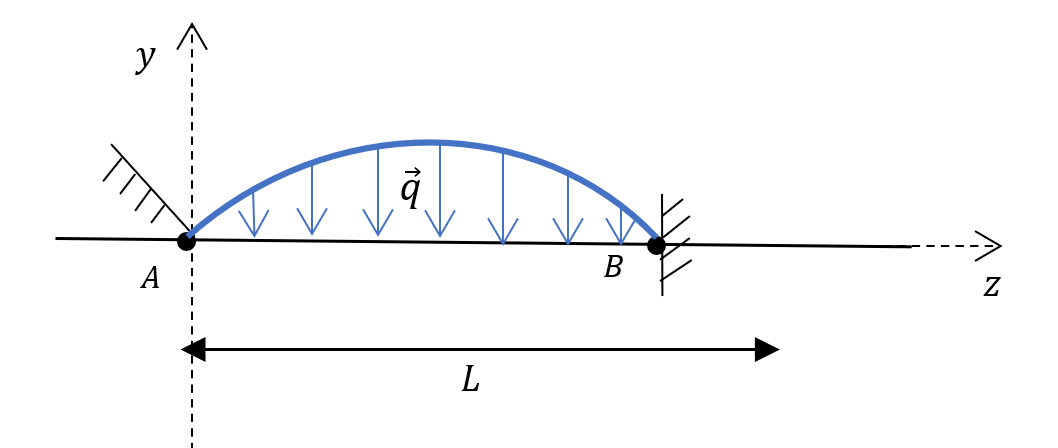
\includegraphics[width=0.5\textwidth]{beam}
		\caption{Закреплённая балка длины $L$}
		\label{fig:beam}
	\end{figure}

Уравнение (\refeq{v1}) должно быть дополнено четырьмя граничными условиями, в качестве которых рассмотрим следующие:
\begin{enumerate} 
\item[1)] $y|_{z=0}=0$ --- отсутствие перемещения в т.$A$;
\item[2)] $y^{'}|_{z=0}=-\frac{\pi}{180}$ --- поворот в т.$A$ на $1^{\circ}$;
\item[3)] $y|_{z=L}=0$ --- отсутствие перемещения в т.$B$;
\item[4)] $y^{'}|_{z=L}=0$ --- отсутствие поворота сечения в т.$B$.
\end{enumerate}


Тогда точное решение уравнения (\refeq{v1}) будет иметь вид: \\
$$y=-\frac{\left(\pi ^4 (z-1)+180\right) (z-1) z}{180 \pi ^3}-\frac{\sin (\pi  z)}{\pi ^4}.$$

Построим график точного решения и отметим на нем узловые перемещения, полученные приближенно при помощи метода конечных элементов в случае трёхузлового КЭ. 

	\begin{figure}[H]
		\centering
		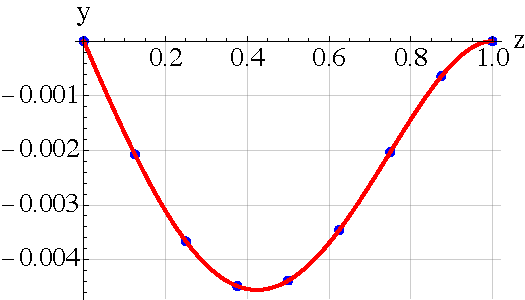
\includegraphics[width=0.5\textwidth]{3_comparison}
		\caption{Сравнение точного и приближенного решения при $n=4$, полученного при помощи МКЭ}
		\label{fig:3_comparison}
	\end{figure}

Посчитаем норму разности точного и приближённого решений дифференциального уравнения в пространстве функций $L_{2}$ и дадим апостериорную оценку порядка точности метода $m$.

\begin{figure}[H]
		\centering
		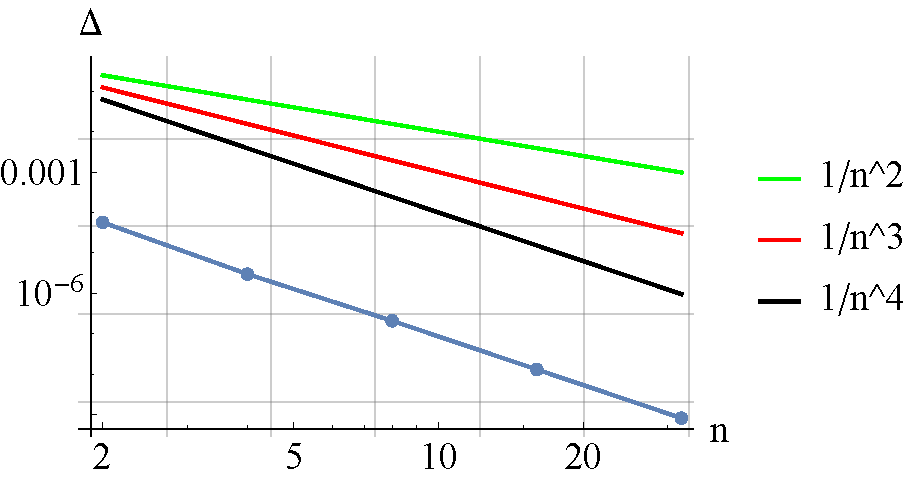
\includegraphics[width=0.55\textwidth]{2_nodebeam_plain}
		\caption{Зависимость погрешности от числа конечных элементов (двухузловой КЭ)}
		\label{fig:2_nodebeam_plain}
	\end{figure}

\[
\begin{array}{|c|c|c|c|c|c|}
\hline
\hline
\text{N} & 2 & 4 & 8 & 16 & 32 \\ \hline
\Delta  & 5.87 \cdot 10^{-5}  & 3.51 \cdot 10^{-9} & 2.17 \cdot 10^{-7} & 1.35 \cdot 10^{-8} & 8.43 \cdot 10^{-10}\\ \hline
m &  & 4.06 & 4.02 & 4.11 & 4.01 \\ 
\hline
\hline
\end{array}
\]

Видно, что при двухкратном увеличении числа КЭ погрешность уменьшается примерно в 16 раз, что означает, что двухузловой конечный элемент имеет 4 порядок точности.

Аналогичный тест проведем для трехузлового конечного элемента и получим следующие значения. 

\begin{figure}[H]
		\centering
		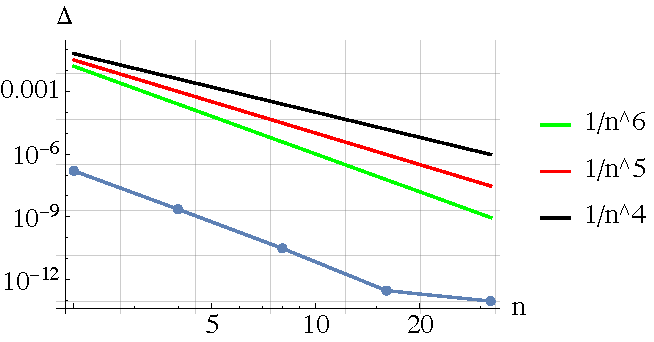
\includegraphics[width=0.55\textwidth]{3_nodebeam_plain}
		\caption{Зависимость погрешности от числа конечных элементов (трехузловой КЭ)}
		\label{fig:3_nodebeam_plain}
	\end{figure}
	
\[
\begin{array}{|c|c|c|c|c|c|}
\hline
\text{N} & 2 & 4 & 8 & 16 & 32 \\ \hline
\Delta  & 1.56 \cdot 10^{-7} & 2.31 \cdot 10^{-9} & 3.13 \cdot 10^{-11} & 3.01 \cdot 10^{-13} & 9.36 \cdot 10^{-14} \\ \hline
m &  & 6.08 & 6.21 & 6.71 & 1.68 \\ 
\hline
\end{array}
\]

Проанализировав зависимость погрешности от числа конечных элементов, изображенную на рис.~\ref{fig:3_nodebeam_plain}, заметим, что точность метода конечных элементов, реализованного для задачи с трехузловым конечным элементом, имеет 6-й порядок. 

Таким образом, метод конечных элементов, реализованный для двухузлового КЭ, в случае гладкой нагрузки $q$, действующей на балку, имеет 4-й порядок точности, а для трехузлового КЭ --- 6-й порядок. 



\subsection[Непрерывная негладкая функция внешней нагрузки]{Непрерывная негладкая функция внешней нагрузки с \glqq изломом \grqq в узле}

Рассмотрим случай, когда внешняя нагрузка $q$, действующая на балку, является непрерывной и негладкой.
 
\[
q = 
 \begin{cases}
   Q \sin \left(\frac{\pi  z}{z_{0}}\right) & z \leq z_{0}, \\
   Q \sin \left(\frac{\pi  (z-z_{0})}{z_{0}}\right) & z > z_{0},
 \end{cases}
\]
где $z_{0}=\frac{L}{2}$ --- точка разрыва, $L$ --- длина балки. \\

На рис.~\ref{fig:q_cont_in} изображён график внешней нагрузки, действующей на балку. Точка разрыва производной попадает в узел конечноэлементной сетки.
	\begin{figure}[H]
		\centering
		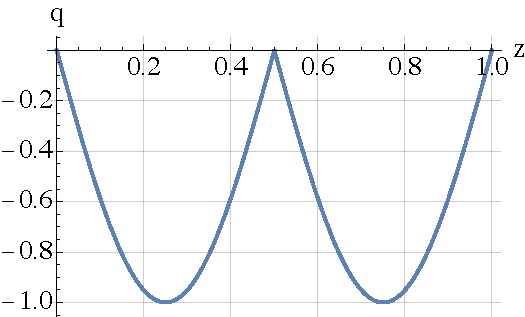
\includegraphics[width=0.5\textwidth]{q_cont_in}
		\caption{Непрерывная негладкая внешняя нагрузка $q$, действующая на балку}
		\label{fig:q_cont_in}
	\end{figure}

%Теперь подставим значение функции внешней нагрузки в уравнение (\refeq{v1}) и получим:\\
%
%\begin{center}
%$(EIy^{''}_{zz})^{''}_{zz}$ = 
% \begin{cases}
%   Q \sin \left(\frac{\pi  z}{z_{0}}\right) & z \leq z_{0}, \\
%   Q \sin \left(\frac{\pi  (z-z_{0})}{z_{0}}\right) & z > z_{0}.
% \end{cases}
%\end{equation}
%\end{center}

Точное решение уравнения будет иметь вид:\\
если $z \leq \frac{1}{2}$\\
$$y(z)= \left(\frac{1}{12 \pi }-\frac{\pi }{180}\right) z^3+\left(-\frac{1}{4 \pi ^3}-\frac{1}{16 \pi }+\frac{\pi }{90}\right) z^2+\left(\frac{1}{8 \pi ^3}-\frac{\pi }{180}\right) z -\frac{\sin (2 \pi  z)}{16 \pi ^4},$$\\
если $z > \frac{1}{2}$\\
$$y(z)= \left(\frac{1}{12 \pi }-\frac{\pi }{180}\right) z^3+\left(-\frac{1}{4 \pi ^3}-\frac{1}{16 \pi }+\frac{\pi }{90}\right) z^2+\left(\frac{1}{8 \pi ^3}-\frac{\pi }{180}\right) z +{}$$
$${} + \frac{3 \sin (2 \pi  z)-\pi  \left(\pi ^2 (1-2 z)^2-6\right) (2 z-1)}{48 \pi ^4}.$$ \\


Оценим норму разности точного и приближённого решений дифференциального уравнения в пространстве функций $L_{2}$  и оценим как эта норма зависит от количества конечных элементов.\\

\begin{figure}[H]
		\centering
		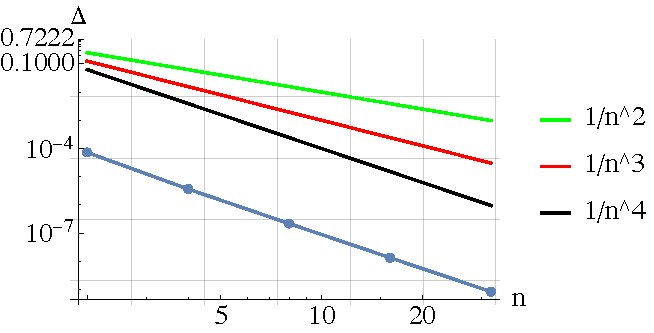
\includegraphics[width=0.55\textwidth]{2_nodebeam_cont_in}
		\caption{Зависимость погрешности от числа конечных элементов (двухузловой КЭ)}
		\label{fig:2_nodebeam_cont_in}
\end{figure}


	
\[
\begin{array}{|c|c|c|c|c|c|}
\hline
\text{N} & 2 & 4 & 8 & 16 & 32 \\ \hline
\Delta  & 7.21 \cdot 10^{-5} & 3.67 \cdot 10^{-6} & 2.21 \cdot 10^{-7} & 1.35 \cdot 10^{-8} & 8.44 \cdot 10^{-10}\\ \hline
m  &  & 4.31 & 4.06 & 4.02 & 4.01 \\ 
\hline
\end{array}
\]



Проанализировав зависмость погрешности от числа конечных элементов, изображенную на рис.~\ref{fig:2_nodebeam_cont_in}, заметим, что точность метода конечных элементов, реализованного для задачи с двухузловым КЭ, имеет 4 порядок. 

Аналогичный тест проведем для трёхузлового конечного элемента. Зависимость погрешности от числа коненчых элементов имеет следующий вид: \\
\begin{figure}[H]
		\centering
		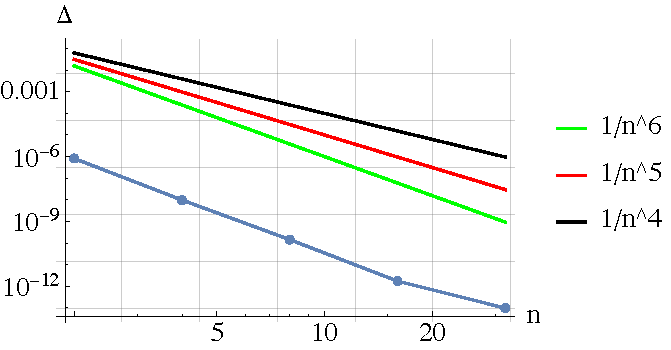
\includegraphics[width=0.55\textwidth]{3_nodebeam_cont_in}
		\caption{Зависимость погрешности от числа конечных элементов (трехузловой КЭ)}
		\label{fig:3_nodebeam_cont_in}
\end{figure}


	
\[
\begin{array}{|c|c|c|c|c|c|}
\hline
\text{N} & 2 & 4 & 8 & 16 & 32\\ \hline
\Delta  & 8.16 \cdot 10^{-7} & 9.81 \cdot 10^{-9} & 1.45 \cdot 10^{-10} & 1.74 \cdot 10^{-12} & 9.82 \cdot 10^{-14}\\ \hline
m &  & 6.38 & 6.08 & 6.38 & 4.14 \\ 
\hline
\end{array}
\]

По зависимости погрешности от числа конечных элементов, изображенную на рис.~\ref{fig:3_nodebeam_cont_in}, видим, что точность метода конечных элементов, реализованного для задачи с трёхузловым конечным элементом, имеет 6 порядок. 

Таким образом, метод конечных элементов, реализованный для двухузлового КЭ, в случае непрерывной и негладкой внешней нагрузки $q$, точка разрыва производной попадает в узел, действующей на балку, имеет 4 порядок точности, а для трехузлового КЭ --- 6 порядок. \\

\subsection{Непрерывная негладкая функция внешней нагрузки с \glqq изломом \grqq не в узле}

Рассмотрим случай, когда внешняя нагрузка $q$ , действующая на балку, является непрерывной негладкой, а точка разрыва производной не попадает в узел.
 
\[
q = 
 \begin{cases}
Q \sin \left(\frac{\pi  z}{z_{0}} \right)   &  z \leq z_{0}, \\
Q \sin \left(\frac{\pi  (z-z_{0})}{z_{0}} \right) & z > z_{0},
 \end{cases}
\]
где $z_{0}=\frac{3L}{7}$ --- точка разрыва, не попадающая в узел,  $L$ --- длина балки. \\

На рис.~\ref{fig:q_cont_out} изображён график внешней нагрузки, действующей на балку.
	\begin{figure}[H]
		\centering
		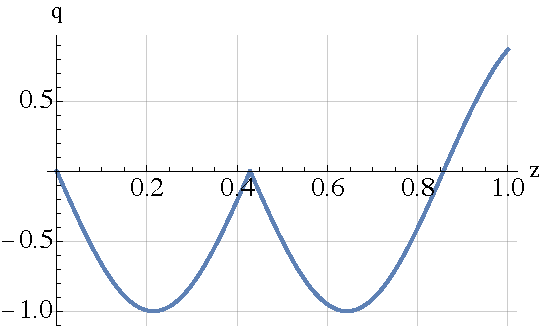
\includegraphics[width=0.5\textwidth]{q_cont_out}
		\caption{Непрерывная и негладкая внешняя нагрузка $q$, действующая на балку}
		\label{fig:q_cont_out}
	\end{figure}

Точное решение уравнения, описывающего форму упругой линии балки, будет иметь вид:\\

Если $z \leq \frac{3}{7}$ 
$$y(z)= \left(\frac{81 \sqrt{3}}{2401 \pi ^4}-\frac{\pi }{180}+\frac{208}{2401 \pi }+\frac{297}{4802 \pi ^3}\right) z^3+\left(-\frac{243 \sqrt{3}}{4802 \pi ^4}-\frac{144}{2401 \pi }-\frac{1107}{4802 \pi ^3}+\frac{\pi }{90}\right) z^2+$$
$$+\left(\frac{27}{343 \pi ^3}-\frac{\pi }{180}\right) z -\frac{81 \sin \left(\frac{7 \pi  z}{3}\right)}{2401 \pi ^4}.$$

Если $z > \frac{3}{7}$
$$  y(z)= \left(\frac{27}{343 \pi ^3}-\frac{\pi }{180}\right) z+\left(-\frac{243 \sqrt{3}}{4802 \pi ^4}-\frac{144}{2401 \pi }-\frac{1107}{4802 \pi ^3}+\frac{\pi }{90}\right) z^2+$$
$$+\left(\frac{81 \sqrt{3}}{2401 \pi ^4}-\frac{\pi }{180}+\frac{208}{2401 \pi }+\frac{297}{4802 \pi ^3}\right) z^3 - \frac{81 \sin \left(\frac{7 \pi  z}{3}\right)-\pi  \left(\pi ^2 (3-7 z)^2-54\right) (7 z-3)}{2401 \pi ^4}.$$ \\

Посчитаем норму разности точного и приближённого решений дифференциального уравнения в пространстве функций $L_{2}$  и оценим как эта норма зависит от количества конечных элементов.\\

\begin{figure}[H]
		\centering
		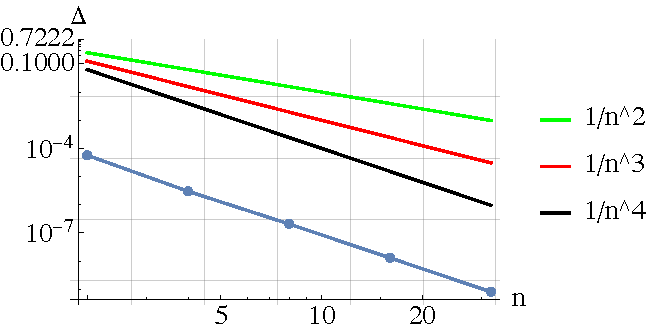
\includegraphics[width=0.55\textwidth]{2_nodebeam_cont_out}
		\caption{Зависимость погрешности от числа конечных элементов (двухузловой КЭ)}
		\label{fig:2_nodebeam_cont_out}
	\end{figure}


\[
\begin{array}{|c|c|c|c|c|c|}
\hline
\text{N} & 2 & 4 & 8 & 16 & 32 \\ \hline
\Delta  & 5.71 \cdot 10^{-7} & 3.11 \cdot 10^{-6} & 2.08 \cdot 10^{-7} & 1.32 \cdot 10^{-8} & 8.11 \cdot 10^{-10}\\ \hline
m  &  &4.25 & 3.85 & 3.90 & 4.01 \\ 
\hline
\end{array}
\]

Проанализировав зависмость погрешности от числа конечных элементов, изображенную на рис.~\ref{fig:2_nodebeam_cont_out}, заметим, что точность метода конечных элементов, реализованного для задачи с двухузловым конечным элементом, имеет 4 порядок. 


Аналогичный тест проведем для трехузлового КЭ, реализованного для задачи с непрерывной и негладкой функцией внешней нагрузки, точка разрыва производной не в узле.  
\begin{figure}[H]
		\centering
		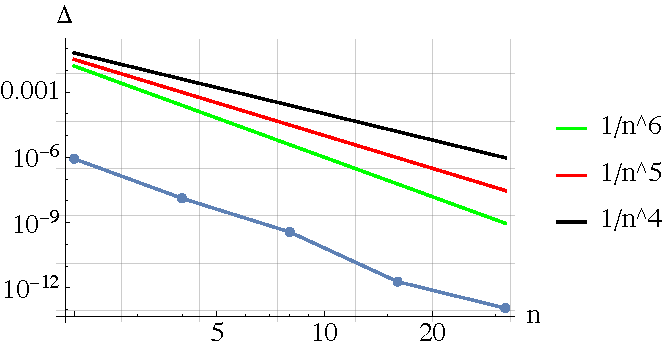
\includegraphics[width=0.55\textwidth]{3_nodebeam_cont_out}
		\caption{Зависимость погрешности от числа конечных элементов (трехузловой КЭ)}
		\label{3_nodebeam_cont_out}
	\end{figure}


\[
\begin{array}{|c|c|c|c|c|c|}
\hline
\text{N} & 2 & 4 & 8 & 16 & 32 \\ \hline
\Delta  & 8.55 \cdot 10^{-7} & 1.31 \cdot 10^{-8} & 3.70 \cdot 10^{-10} & 1.94 \cdot 10^{-12} & 1.18 \cdot 10^{-13}  \\ \hline
m  & & 6.03 & 5.15 & 7.57 & 4.03 \text{} \\ 
\hline
\end{array}
\]

По графику можно заметить, что точность метода коненчных элементов для трёхузлового КЭ, в случае непрерывной негладкой функции внешней нагрузки с разрывом не в узле, имеет 6 порядок.\\





\subsection[Ограниченная функция внешней нагрузки с \glqq изломом \grqq в узле]{Ограниченная разрывная функция внешней нагрузки с \glqq изломом \grqq в узле}

Рассмотрим случай, когда внешняя нагрузка, действующая на балку $q$ является разрывной, но ограниченной, причем функция имеет разрыв в узле, а не между узлами, а значит при измельчении сетки каждый узел попадает в точку приложения нагрузки. \\

 Тогда функция внешней нагрузки имеет следующий вид:

\begin{equation}
q = 
 \begin{cases}
	Q \sin \left(\frac{\pi  z}{z_{0}}\right) & z \leq z_{0},\\
    Q \sin \left(\frac{\pi  (z-z_{0})}{z_{0}}\right) & z > z_{0}.
 \end{cases}
\end{equation}

где $z_{0}=\frac{L}{2}$ --- точка разрыва, совпадающая с узлом сетки, $L$ --- длина балки. \\

Посчитаем норму разности точного и приближённого решений дифференциального уравнения в пространстве функций $L_{2}$  и оценим как эта норма зависит от количества конечных элементов.\\

\begin{figure}[H]
	\centering
	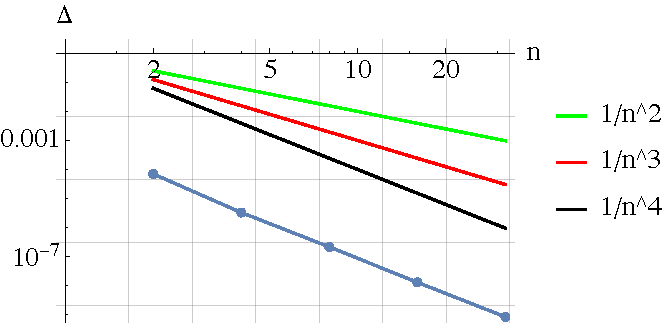
\includegraphics[width=0.55\textwidth]{2_nodebeam_cont_finite_in}
	\caption{Зависимость погрешности от числа конечных элементов (двухузловой КЭ)}
	\label{fig:2_nodebeam_cont_finite_in}
\end{figure}
\[
\begin{array}{|c|c|c|c|c|c|}
	\hline
	\text{N} & 2 & 4 & 8 & 16 & 32 \\ \hline
\Delta  & 7.1 \cdot 10^{-5} & 3.3 \cdot 10^{-6} & 2.2 \cdot 10^{-7} & 1.3 \cdot 10^{-8} & 8.4 \cdot 10^{-10}\\ \hline
m  &  & 4.41 & 3.94 & 4.06 & 3.95 \\ 
	\hline
	\end{array}
	\]

Проанализировав полученный результат, заметим, что при двухкратном увеличении числа КЭ погрешность уменьшается примерно в 16 раз, что означает, что метод имеет 4-й порядок точности.\\

 Проведем тест для трехузлового конечного элемента и получим следующие значения. 
\begin{figure}[H]
		\centering
		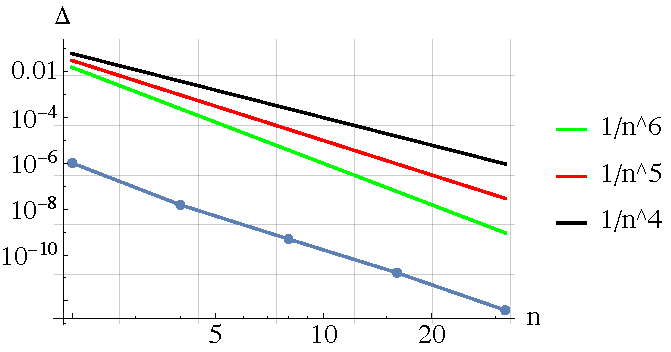
\includegraphics[width=0.55\textwidth]{3_nodebeam_cont_finite_in}
		\caption{Зависимость погрешности от числа конечных элементов (трехузловой КЭ)}
		\label{fig:3_nodebeam_cont_finite_in}
	\end{figure}


\[
\begin{array}{|c|c|c|c|c|c|}
\hline
\text{N} & 2 & 4 & 8 & 16 & 32 \\ \hline
\Delta  & 1.04 \cdot 10^{-6} & 1.55 \cdot 10^{-8} & 4.9 \cdot 10^{-10} & 1.689 \cdot 10^{-11} & 3.9 \cdot 10^{-13} \\ \hline
m  &  & 6.07 & 4.96 & 4.88 & 5.43 \\ 
\hline
\end{array}
\]
По графической зависимости видим, что точность метода конечных элементов, реализованного для задачи с трехузловом КЭ конечным элементом, имеет 6 порядок. 

Таким образом, метод конечных элементов, реализованный для двухузлового КЭ, в случае разрывной и ограниченной внешней нагрузки $q$, имеющей разрыв в узле, действующей на балку, имеет 4 порядок точности, а для трехузлового КЭ --- 6 порядок. 




\subsection[Ограниченная функция внешней нагрузки с \glqq изломом \grqq не в узле]{Ограниченная разрывная функция внешней нагрузки с \glqq изломом \grqq не в узле}

Рассмотрим случай, когда внешняя нагрузка, действующая на балку $q$ является разрывной, но ограниченной, причем функция имеет разрыв между узлами. 
Тогда функция внешней нагрузки имеет следующий вид:

\begin{equation}
q = 
 \begin{cases}
	Q \sin \left(\frac{\pi  z}{z_{0}}\right) & z \leq \frac{8 z_{0}}{10}, \\
    Q \sin \left(\frac{\pi  (z-z_{0})}{z_{0}}\right) & z > \frac{8 z_{0}}{10},
 \end{cases}
\end{equation}
где $z_{0}=\frac{L}{2}$ --- точка разрыва, $L$ ---длина балки. 
Посчитаем норму разности точного и приближённого решений дифференциального уравнения в пространстве функций $L_{2}$  и оценим как эта норма зависит от количества конечных элементов.\\

\begin{figure}[H]
		\centering
		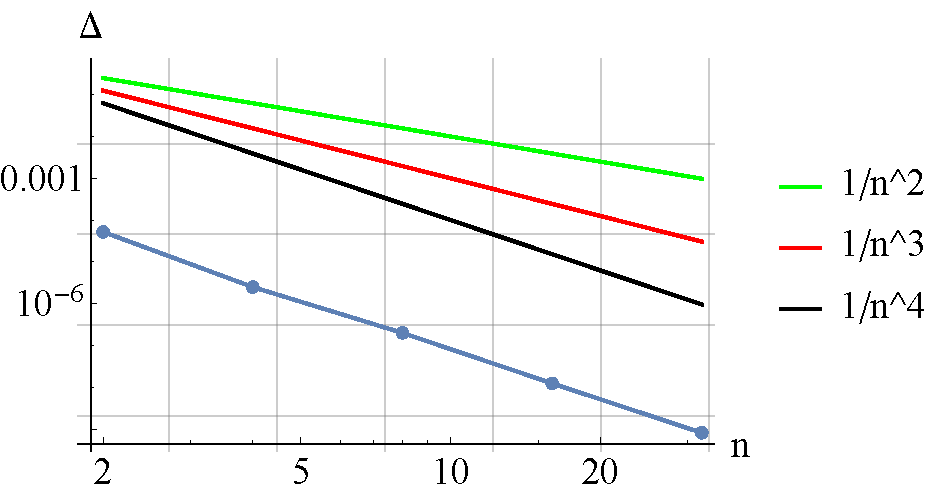
\includegraphics[width=0.55\textwidth]{2_nodebeam_cont_finite_out}
		\caption{Зависимость погрешности от числа конечных элементов (двухузловой КЭ)}
		\label{fig:2_nodebeam_cont_finite_out}
	\end{figure}

\[
\begin{array}{|c|c|c|c|c|c|}
\hline
\text{N} & 2 & 4 & 8 & 16 & 32 \\ \hline
\Delta  & 5.21 \cdot 10^{-5} & 2.50 \cdot 10^{-6} & 1.92 \cdot 10^{-7} & 1.23 \cdot 10^{-8} & 8.12 \cdot 10^{-10} \\ \hline
m  &  & 4.38 & 3.64 & 4.01 & 3.92 \\ 
\hline
\end{array}
\]

Проанализировав полученный результат, заметим, что при двухкратном увеличении числа КЭ погрешность уменьшается примерно в 16 раз, что означает, что метод имеет 4-й порядок точности.\\


 Проведем тест для трехузлового конечного элемента и получим следующие значения. 
\begin{figure}[H]
		\centering
		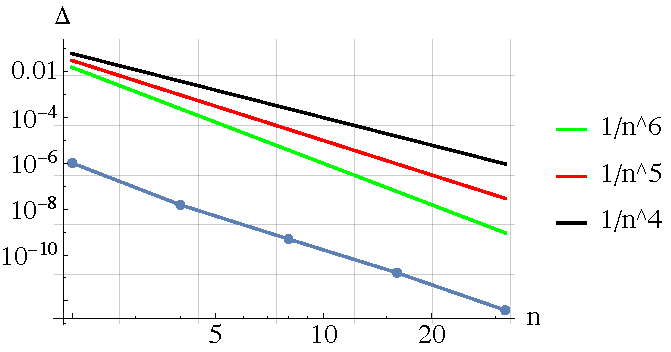
\includegraphics[width=0.55\textwidth]{3_nodebeam_cont_finite_out}
		\caption{Зависимость погрешности от числа конечных элементов (трехузловой КЭ)}
		\label{fig:3_nodebeam_cont_finite_out}
	\end{figure}


\[
\begin{array}{|c|c|c|c|c|c|}
\hline
\text{N} & 2 & 4 & 8 & 16 & 32\\ \hline
\Delta  & 1.02 \cdot 10^{-6} & 3.25 \cdot 10^{-8} & 5.93 \cdot 10^{-10} & 9.64 \cdot 10^{-12} & 1.39 \cdot 10^{-13}\\ \hline
m  &  &  4.96 & 5.78 & 5.94 & 6.12 \\ 
\hline
\end{array}
\]

По графической зависимости видим, что точность метода конечных элементов, реализованного для задачи с 	трехузловым конечным элементом, имеет 4 порядок, т.к. при двухкратном увеличении числа коненчных элементов, погрешность уменьшается примерно в 64 раза. 


Таким образом, метод конечных элементов, реализованный для двухузлового КЭ, в случае разрывной и ограниченной внешней нагрузки $q$, имеющей разрыв не в узле, действующей на балку, имеет 4 порядок точности, а для трехузлового КЭ --- 6 порядок. 

\subsection[Сосредоточенная функция внешней нагрузки]{Сосредоточенная не в узле функция внешней нагрузки}

Рассмотрим случай,когда сосредоточенная нагрузка приложена не к узлу, а между узлами (точка выбрана так, чтобы при измельчении сетки ни один не узел в точку приложения нагрузки не попадал).  \\

Тогда функция внешней нагрузки имеет следующий вид:

$$q = 10 Q L  \delta (z - z_{0}),$$

где $z_{0}=\frac{3L}{7}$ --- точка, в которой действует сосредоточенная нагрузка, не совпадающая с узлом сетки, $\delta$ --- дельта-функция Дирака, $L=1$ --- длина балки. \\

Точное решение уравнения будет иметь вид:
$$
	y(z)= z^3 \left(-\frac{1}{3} 5 H (7 z-3)-\frac{\pi }{180}+\frac{1040}{1029}\right)+z^2 \left(\frac{15 H (7 z-3)}{7}-
-\frac{240}{343}+\frac{\pi }{90}\right)+$$
$$+z \left(-\frac{1}{49} 45 H (7 z-3)-\frac{\pi }{180}\right)+\frac{45 H (7 z-3)}{343},
$$
%$$y(z)= z^3 \left(-\frac{1}{3} 5 H (7 z-3)-\frac{\pi }{180}+\frac{1040}{%^1029}\right)+z^2 \left(\frac{15 H (7 z-3)}{7}-
%-\frac{240}{343}+\frac{\pi }{90}\right)+ $$\\
%$$+z \left(-\frac{1}{49} 45 H (7 z-3)-\frac{\pi }{180}\right)+\frac{45 H (7 z-3)}{343},$$

где $H$ --- функция Хевисайда.\\

Посчитаем норму разности точного и приближённого решений дифференциального уравнения в пространстве функций $L_{2}$  и оценим как эта норма зависит от количества конечных элементов.\\

\begin{figure}[H]
		\centering
		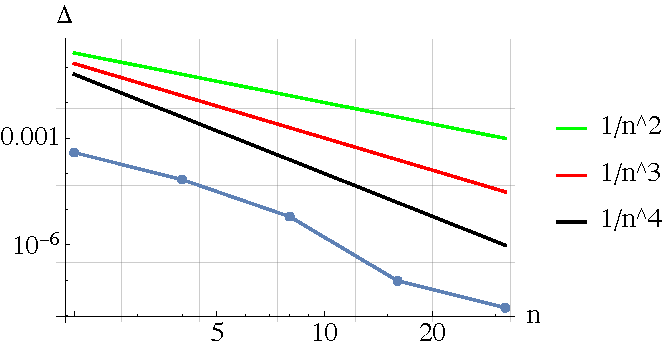
\includegraphics[width=0.55\textwidth]{2_nodebeam_concentrated_out}
		\caption{Зависимость погрешности от числа конечных элементов (двухузловой КЭ)}
		\label{fig:2_nodebeam_concentrated_out}
	\end{figure}

\[
\begin{array}{|c|c|c|c|c|c}
\hline
\text{N} & 2 & 4 & 8 & 16 & 32\\ \hline
\Delta  &3.91 \cdot 10^{-4} & 6.72 \cdot 10^{-5} & 6.11 \cdot 10^{-6} & 9.53 \cdot 10^{-8} & 1.65 \cdot 10^{-8} \\ \hline
m  &  & 2.52 & 3.47 & 6.00 & 2.52 \\ 
\hline
\end{array}
\]

Построим график зависимости нормы разности точного и приближённого решений дифференциального уравнения в пространстве функций $L_{2}$ точного и приближенного решения и числа конечных элементов случае трёхузлового конечного элемента. 

	\begin{figure}[H]
		\centering
		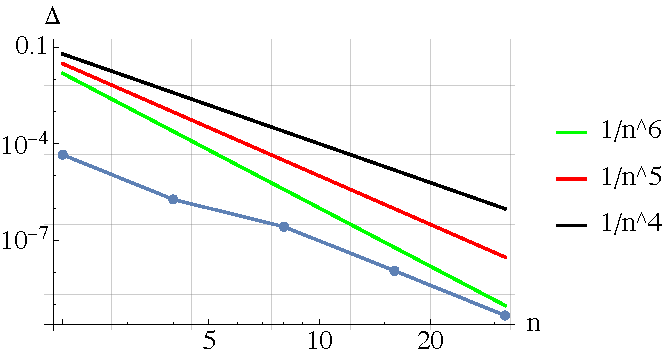
\includegraphics[width=0.55\textwidth]{3_nodebeam_concentrated_out}
		\caption{Сравнение точного и приближенного решения при $n=4$ , полученного при помощи МКЭ (трехузловой КЭ)}
		\label{fig:3_nodebeam_concentrated_out}
	\end{figure}

\[
\begin{array}{|c|c|c|c|c|c|}
\hline
\text{N} & 2 & 4 & 8 & 16 & 32\\ \hline
\Delta  & 4.52 \cdot 10^{-5} & 1.86 \cdot 10^{-6} & 2.64 \cdot 10^{-7} & 1.12 \cdot 10^{-8} & 4.54 \cdot 10^{-10} \\ \hline
m  &  &  4.62 & 2.82 & 4.56 & 4.62 \\ 
\hline
\end{array}
\]
 По построенным графикам зависимости погрешности от числа конечных элементов, заметим, что как в случае двухузлового, так и в случае трехузлового КЭ, порядок точности близок к четвертому. 
\newpage

    \section-{Заключение}
В работе рассмотрена задача о поиске статического прогиба упругой соответствующим образом закрепленной балки, сводящаяся к решению краевой задачи для обыкновенного дифференциального уравнения 4-го порядка. В ходе выполнения курсовой работы освоена технология метода конченых элементов для решения указанной задачи. Рассмотрены двухузловые и трехузловые конечные элементы, для модельных задач, имеющих точные аналитические решения, получены оценки порядка точности для различной степени гладкости правой части уравнения (функции внешней нагрузки). 
		
		\newpage

\begin{thebibliography}{9}
	\bibitem{book0} Светлицкий В.\,А. Механика гибких стержней и нитей. М.: Машиностроение, 1978. 213 с.
	\bibitem{book1} Зенкевич О. Метод конечных элементов в технике / пер. Б.Е. Победри. М.: Мир, 1975. 540 с.
	\bibitem{book2} Галанин М. \,П., Савенков Е. \,Б. Методы численного анализа математических моделей  - 2-е изд., испр. - М. : Изд-во МГТУ им. Н. Э. Баумана, 2018. - 591 с. 
\end{thebibliography}
		
		
 

\end{document}